\chapter{Introduction}
\label{chap:intro}

The advancement of gaming device technology such as Kinect, Wii Balance Board, Wii Remote, PlayStation Move, etc. has enabled players to control and interact with the game console through body movement. In healthcare, such technologies are used in serious game which can help users (doctors, patients, researchers, etc.)  perform health related activity such as patients' rehabilitation and training\cite{rahman,brezinka,green}. One example of such game is Hammer and Planks. Developed by NaturalPad\footnote{\url{www.naturalpad.fr}}, Hammer and Planks was designed to train the equilibrium of patient with balance disorders (specifically for hemiplegic people)\cite{diloreto}. A person with hemiplegic is paralized on one side of the body\footnote{\url{http://www.hemihelp.org.uk/hemiplegia/what_is_hemiplegia}}. Therefore, the gameplay is designed so that the player has to move their body to the right, left, forward and backward in order to train their affected side of the body. To support the purpose of rehabilitation, the healthcare professionals need to analyse the movement to  make a correct diagnostic of patients' progress and to adjust the difficulty level for the next rehabilitation session. In this thesis, we discuss the design of an interface to help healthcare professional understand the data generated from the game.

\section{Motivation}

Hammer and Planks is a vertical shooter game. The game world is in a 2D environment vertically scrolling from top to bottom in which a player navigate a ship from left to right through moving his body. It tells the story of a pirate named John K. One day a meteor fell down on John's ship and ruin it. There is a little left from his boat but it is still enough to build a new basic boat with what's left. While navigating his ship to collect driftwood/plank to upgrade it (hence the name Hammer and Planks), he also wants to find the ship which showered meteor and destroyed his ship. Therefore, in the game a player has to defeat all enemies which come on his way and he has to avoid being destroyed by bullets, reefs and other obstacles. Throughout the game the player has to collect bonuses (planks) to improve the ship. The game is usually played in short and intense phase and thus requires a lot of concentration\cite{diloreto}. Figure \ref{game_screenshot} shows the interface of the game. The boat in the middle represents the player, the reefs are obstacles which should be avoided, driftwood/planks shown in yellow circle are bonuses which should be collected, and the object emanating fires is an enemy which should be killed.

Currently, the game provides some charts which visualize player's body movement with respect to the horizontal axis and vertical axis (Figure \ref{current_viz}). However, the information that can be gathered from the visualization is not enough for the healthcare professional to be able to establish an informed diagnostic. It's hard to know how often the player move to the right or left. It's also not possible to know to which type of events (ie. avoiding an enemy, catching the bonuses) the movement is related to. Which is crucial since the therapist need to know if the player is able to develop strategy to play the game overtime. The existing visualization also provides chart to show the evolution of player's performance and total movement for all game sessions. However, the evolution of player's body movement is not depicted.

\begin{figure}[H]
\centering
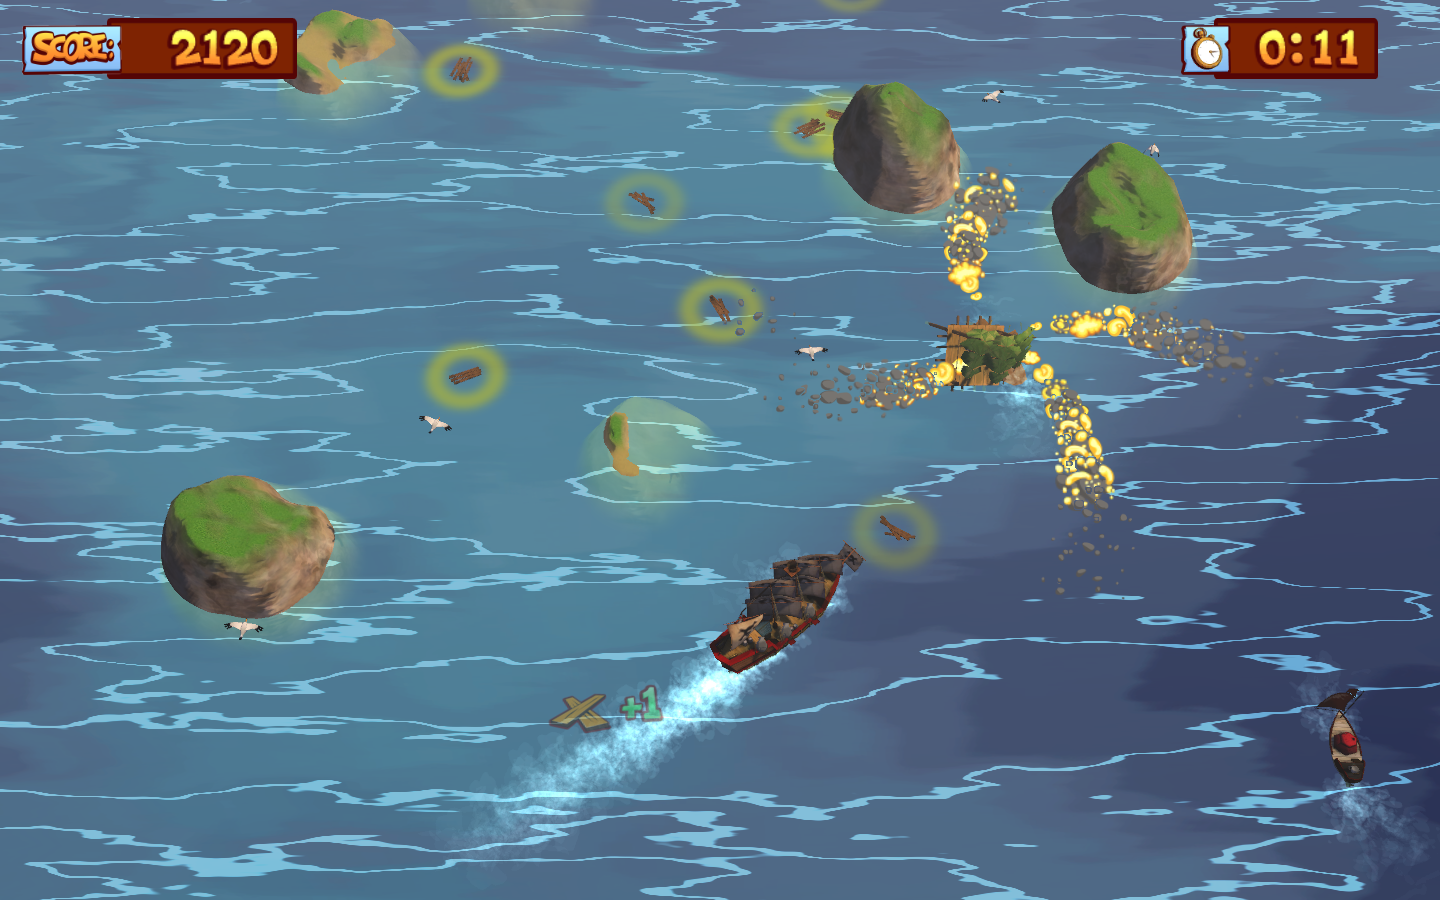
\includegraphics[width=110mm]{hp_game.png}
\caption{Hammer and Planks Screenshot \label{game_screenshot}}
\end{figure}

\begin{figure}[H]
\centering
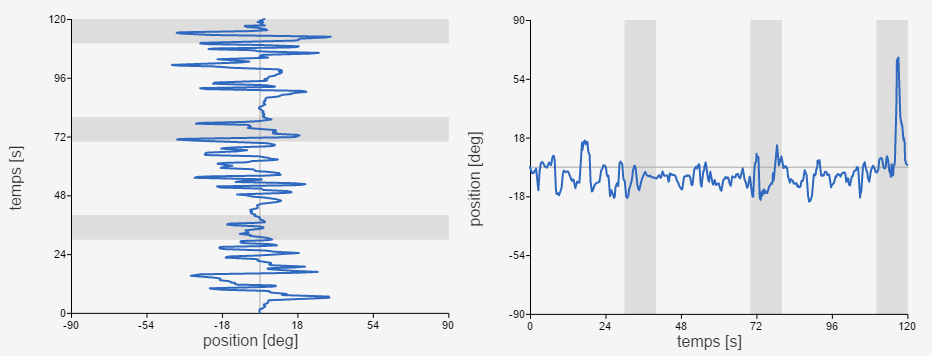
\includegraphics[width=130mm]{current_viz.png}
\caption{Current visualization used in the game to show movements over horizontal and vertical axis \label{current_viz}}
\end{figure}

The purpose of this thesis is to address the problem mentioned by proposing a visualization interface to help healthcare professionals analyse gameplay data generated from the game so that they can determine the frequency and direction of player movement as well as movement pattern evolution over time. It is important for the interface to be simple and intuitive but at the same time still able to correctly shows the information needed by healthcare professionals. In this case, the visualization design process is difficult due to the heterogeneity and the size of the data. For instance, Hammer and Planks produces log file with tens of thousands records. Another challenge is how to visualize movement data that can be interpreted intuitively. Currently, there have been several approaches proposed on how to perform visual analytics on movement data. However, most of them deal with "geographical" movements \cite{adrienko_book} and only a few has been dealing with human body movement \cite{bernard2013}. It is also challenging to identify interesting movement pattern from the data as well as choosing the right approach to visualize changes of pattern.
\section{Methodology}

To ensure that the visualization to be designed would satisfy the information needed by healthcare professionals, we followed the Nested Process Model proposed by Tamara Munzner \cite{Munzner:2009:NMV:1638611.1639181}. The model is divided into 4 levels: Domain Problem Characterization, Data/Operation Abstraction Design, Encoding/Interaction Technique Design, and Algorithm Design. These levels are nested; the output of a higher level will be the input for the lower level as shown in Figure \ref{munzner_model}.

\begin{figure}[H]
\centering
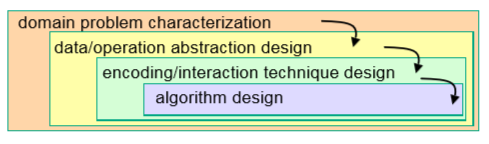
\includegraphics[width=100mm]{munzner_model.png}
\caption{Munzner's Visualization Design Model with four nested layers \label{munzner_model}}
\end{figure}

In domain problem characterization level, the types of information needed by health professional from the visualization are defined. The output of this level would be a list of tasks that need to be solved by the visualization application. We then identify data structures which can support these tasks in the Data/Operation Abstraction Design level. In the third level, a good visualization and interaction techniques which can support the tasks are defined. At last in Algorithm Design level, an algorithm to support the visualization is proposed.

\section{Contribution}
In this thesis, we proposed a visualization interface for healthcare professionals to visualize Hammer and Planks gameplay data to help them analyse player movement during the game as part of rehabilitation process. The visualization provides two type of visualizations:
\begin{itemize}
\item A visualization which provides information on frequency and direction of body movements which are related to objects in the game for one game session.
\item An interactive visualization where healthcare professionals can analyse the evolution of player's body movement throughout all sessions. Here, we proposed an approach to easily navigate and highlight movement pattern. We also proposed a clustering algorithm based on hierarchical clustering to identify similar movement pattern. A distance function is defined to quantify movement pattern similarity which consider both movement evolution and proportion of movement frequency.
\end{itemize}

\section{Thesis Outline}

The remainder of this thesis is organized as follows. Chapter 2 discuss the domain problem characterization. Chapter 3 explores related work. The data abstraction is presented in Chapter 4. The Visual Mapping and Interactive Functionality of the proposed visualization are discussed in details in Chapter 5. Chapter 6 provides some case studies used to evaluate the approach and finally, chapter 7 concludes the thesis.
